The final paper does not focus on GWAS, but rather on the predictive value of the LT-FH++ phenotype as an alternative to the conventional binary family history variable in prediction models. In epidemiology, family history is a well-known and powerful predictor that has been used to improve prediction models of complex phenotypes such as mental disorders and suicide. As the intension is to provide an estimate of an individual's liability for a given disorder before getting an actual diagnosis, we will not consider the case-control status of the index person, but only the family members. In many ways this is similar to the purpose of the PRS and how it is currently being used to screen individuals for disorders. However, instead of using the individual's genotypes to acquire an aggregate genetic risk score, we will use the family history to estimate a liability. 

\subsubsection{Real-world analysis}

\begin{wrapfigure}{O}{10cm}
	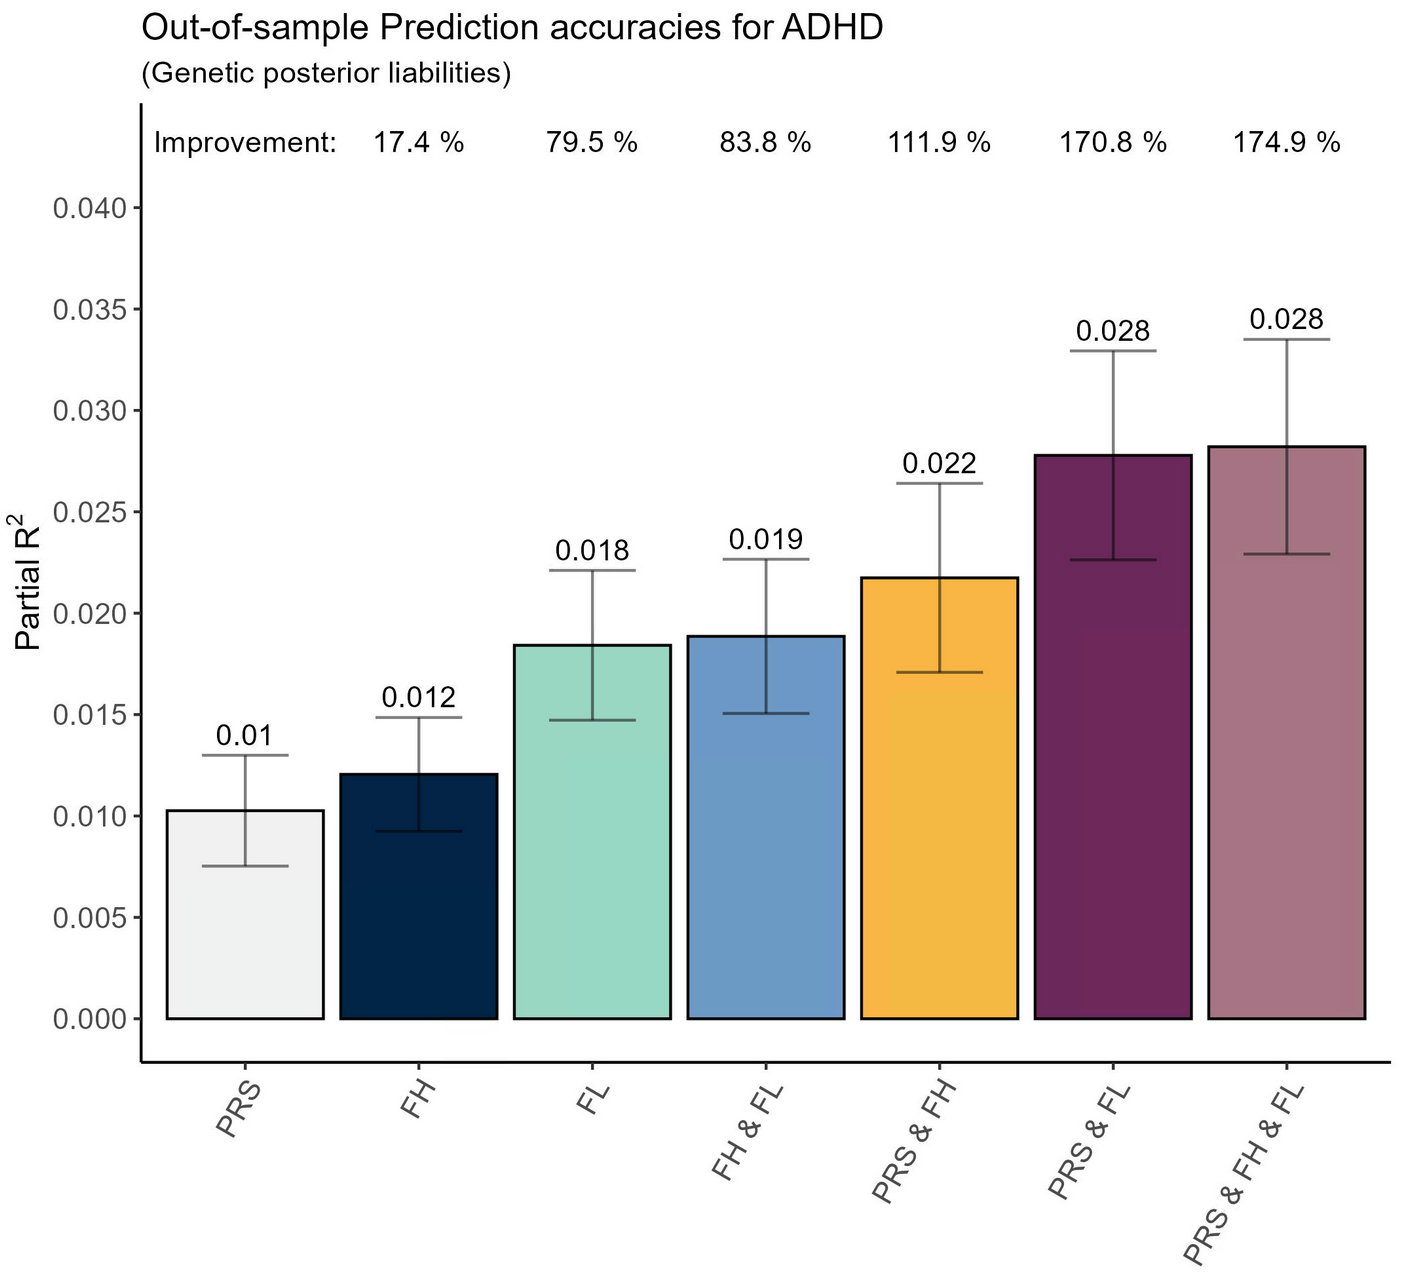
\includegraphics[width=10cm]{results/adhd_predictive_power.png}
	\caption[Out of sample prediction performance]{text}
	\label{fig:paper3:predictionResults}
\end{wrapfigure}
We will consider a base model that contains the index person's sex, age, and $ 20 $ PCs. We will add additional predictors to the base model and assess the additional predictive value of each predictor. From the additional predictors and combinations of them, we can derive the best family history variable and the best overall model. We will consider the PRS for a given disorder, as well as a binary family history indicator or the LT-FH++ phenotype (but with the index person's status removed). We present the results in \cref{fig:paper3:predictionResults}. The \textbf{TODO: get the average results} average across $ 10 $ phenotypes result in an increased predictive value for both family history variables over the PRS. We find that the LT-FH++ phenotype provided a \textbf{TODO: percent increase over FH} increase over the binary family history variable. The model that performed the best was the model with the PRS and LT-FH++ phenotype with an average partial $ R^2 $ of \textbf{TODO: value}, almost resulting in a partial $ R^2 $ value that is the sum of each predictor. 

On top of this, we will also considered correlated phenotypes. Mental disorders are notoriously difficult to diagnose and many mental disorders have a high genetic correlation. Accounting for correlated phenotypes is therefore an attempt at utilising the information from the highly correlated phenotypes to improve prediction. The multi trait results are presented in \cref{fig:paper3:predictionResultsMultiTrait}. In order to have as fair of a comparison as possible, we also included the values from the correlated phenotypes for the other variables, such as multi trait PRS is a model with the PRS of all the considered correlated phenotypes. Similarly, the binary family history variable for all the correlated phenotypes was also included. For LT-FH++, we considered two scenarios. The first is the correlated phenotype extension as presented in \textbf{TODO: reference relevant method section}. It resulted in a single liability estimate that represents the family history for all of the considered disorders. We also considered a simpler approach, where the single trait LT-FH++ phenotype was included for each of the considered phenotypes.

\begin{wrapfigure}{O}{10cm}
	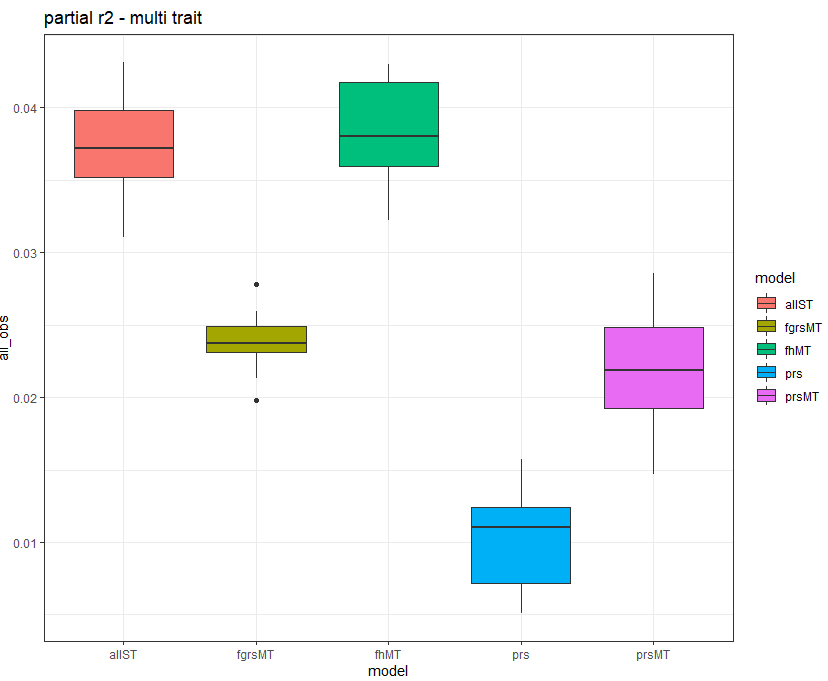
\includegraphics[width=10cm]{results/adhd_predictive_power_multitrait.png}
	\caption[Out of sample multi trait prediction performance]{\textbf{TODO: Very temporary plot.}}
	\label{fig:paper3:predictionResultsMultiTrait}
\end{wrapfigure}


In the multi trait scenario, the LT-FH++ multi trait extension does not perform as well as multiple simple binary family history variables, but it still performs far better than a single PRS, and on par with the PRS of all correlated phenotypes. The most predictive family history model is either the model with all the binary family history variables or all the LT-FH++ phenotypes.


